\chapter{Sampling}

One motivation for conducting quantitative research is to be able to make statements that are representative of reality. Often, studying an entire population is prohibitively expensive or time-consuming, so researchers will select a subset, called a sample, from the population. Under certain conditions, properties of a sample will also hold for the population in general.

\begin{definition}[Inductive statistics]
  Researching properties of a population through sampling is called \emph{inductive statistics}\index{statistics!inductive}.
\end{definition}

\begin{figure}
\centering
  \begin{tikzpicture}[xscale=4,yscale=2]
    \draw (0,2) -- (0,0);
    \foreach \num/\label in {0/0, 0.2/20, .4/40, .6/60, .8/80, 1/100, 1.2/120, 1.4/140, 1.6/160, 1.8/180, 2/200}{%
      \draw (0, \num) -- (2.5, \num);
      \draw[shift={(0, \num)}] (1pt,0pt) -- (-1pt,0pt) node[left] {\scriptsize \label};
    }

    \node[anchor=north] (hero1) at (0.3,1.5)
    {
\includegraphics[height=2.9cm]{images/les2-hero-1}};
    \node[anchor=north] (hero2) at (0.8,2.05)
    {
\includegraphics[height=4cm]{images/les2-hero-2}};
    \node[anchor=north] (hero3) at (1.3,1.575)
    {
\includegraphics[height=3.1cm]{images/les2-hero-3}};
    \node[anchor=north] (hero4) at (1.8,2.1)
    {
\includegraphics[height=4.1cm]{images/les2-hero-4}};
    \node[anchor=north] (hero5) at (2.3,1.95)
    {
\includegraphics[height=3.8cm]{images/les2-hero-5}};

    \node (size1) at (0.3, 1.5) {\scriptsize 141 cm};
    \node (size2) at (0.8, 2.1) {\scriptsize 198 cm};
    \node (size3) at (1.3, 1.51) {\scriptsize 143 cm};
    \node (size4) at (1.8, 2.15) {\scriptsize 201 cm};
    \node (size5) at (2.3, 1.95) {\scriptsize 184 cm};
  \end{tikzpicture}
  \caption{The superheroes being researched.}
  \label{fig:superheldenSteekproef}
\end{figure}

\begin{figure}
  \centering
  
\includegraphics[width=0.85\textwidth]{images/les5-heroes.jpg}
  \caption{The superheroes being researched are only a sample from the population of all superheroes.}
  \label{fig:populatieHelden}
\end{figure}

\section{Population and sample}
\label{sec:population-and-sample}

\begin{definition}[Population]
  The set of \emph{all} items that are being researched is called the \emph{population}\index{population}.
\end{definition}

\begin{definition}[Sample]
  A subset from the population that is being researched more closely is called a \emph{sample}\index{sample}.
\end{definition}

\begin{definition}[Sampling frame]
  The \emph{sampling frame}\index{sampling frame} is a list of all members of the population.
\end{definition}

There are several reasons for using sampling:

\begin{itemize}
  \item The population is too large to do a complete census;
  \item Taking measurements is too expensive;
  \item When timing is an issue, a census may take too long;
  \item It's easier\dots
\end{itemize}

The sampling process consists of several stages:

\begin{enumerate}
  \item \textbf{Defining the population}: Who is part of the population? This is closely related to the problem statement. It's an important step that should not be taken lightly. Elements of note include a.o.~social, demographic or physical properties like gender, age, place of residence, etc.
  
  \item Specifying the \textbf{sampling frame}: Generating a list of the members of the population. For a political opinion poll, this may be an electoral register.
  
  \item Choosing a suitable \textbf{sampling method} and sample size: See Section~\ref{sec:choosing-a-sampling-method}.
\end{enumerate}

\section{Choosing a sampling method}
\label{sec:choosing-a-sampling-method}

\begin{definition}
  A \emph{random sample}\index{sample!random} (also: probability sample\index{sample!probability}) is a selection from the population where each individual has an equal probability of being selected.
\end{definition}

An important result in statistics is that under the assumption that a sample is truly random and the sample is sufficiently large, results for that sample will hold for the entire population.

A \emph{non-probability sample}\index{sample!non-probability} does \emph{not} have this property. Consequently, results within the sample \emph{cannot} be generalised.

\subsection{Stratified sampling}

Often, the population that is being studied is very heterogeneous and differs in important properties (e.g. demographics). In this case, the population may be partitioned into non-overlapping and homogenous classes or \emph{strata}. Examples are a.o.~gender, age categories, income range, or educational level.

\begin{definition}[Stratified Sample]
A \emph{stratified}\index{sample!stratified} sample is proportional when the share of the subpopulation in the sample is proportional to the share in the entire population.
\end{definition}

\begin{example}
  Table~\ref{tab:heldenPopulatie1} gives the frequencies of age and gender in the population of superheroes. Since a census among the superheroes is infeasible, we decide to take a stratified sample. Table~\ref{tab:heldenPopulatie2} gives an example where the size of each stratum is proportional to the group's size in the population.
\end{example}

  \begin{table}
  \centering
    \begin{tabular}{l|cccc|c}
      & \multicolumn{4}{c|}{\textbf{Age}} & \\
      Gender & $\le 18$ & $]18,25]$ & $]25, 40]$ & $> 40$ & Total\\
      \hline
      Female & 500 & 1500 & 1000 & 250 & 3250 \\
      Male   & 400 & 1200 & 800 & 160 & 2560\\
      \hline
      Total  & 900 & 2700 & 1800 & 410 & 5810
    \end{tabular}
    \caption{Frequencies of the superheroes in the population according to gender and age categories.}
    \label{tab:heldenPopulatie1}
\end{table}

\begin{table}
  \centering
    \begin{tabular}{l|cccc|c}
      & \multicolumn{4}{c|}{\textbf{Age}} & \\
      Gender & $\le 18$ & $]18,25]$ & $]25, 40]$ & $> 40$ & Total\\
      \hline
      Female & 50 & 150 & 100 & 25 & 325 \\
      Male   & 40 & 120 & 80 & 16 & 256\\
      \hline
      Total & 90 & 270 & 180 & 41 & 581
    \end{tabular}
      \caption{Stratified sample of the superhero population.}
    \label{tab:heldenPopulatie2}
  \end{table}


\subsection{Sample errors}
\label{ssec:sample-errors}

\paragraph{Random sampling errors}

Random variations in the sampling due to random selection

\paragraph{Systematic sampling errors}

Or selection bias. An example could be an online survey: members of the population without an internet connection cannot participate, so the sample will not be completely random.

\paragraph{Random non-sampling errors}

This includes a.o.~wrong answers or differences in interpretation of the questions.

\paragraph{Systematic non-sampling errors}

Members of the population that have a positive affinity with the research subject (or with science and research in general) are more inclined to participate and will respond with more positive answers. These will not be representative for the entire population.

\subsection{Sample standard deviation}
\label{ssec:sample-standard-deviation}

While the mean over the entire population is notated $\mu$, the \emph{sample mean}\index{mean!sample} is notated as $\overline{x}$ (see also Definition~\ref{def:mean}). Likewise, the sample standard deviation\index{standard deviation!sample} is notated $s$ instead of $\sigma$ (= the population standard deviation).

For the calculation of the sample variance\index{variance!sample}, the formula from Equation~\ref{eq:variance} is adapted:

\begin{equation}
  \label{eq:sample-variance}
  s^2 = \frac{1}{n-1} \sum_{i=1}^{n} (\overline{x} - x_i)^{2}
\end{equation}

Specifically, the denominator of the fraction is $(n-1)$ instead of $n$ (the sample size). 

Since the sum of differences $x_{i} - \overline{x}$ will always be 0 (see Equation~\ref{eq:sumGemid}), and the last difference can be calculated from the first $n-1$ differences. That is, we're not calculating the average deviations of $n$ independent numbers. Only $n-1$ of the squared differences can ``vary freely''. The number $n-1$ is also called the \emph{degrees of freedom}\index{degrees of freedom} of the variance or standard deviation.

\begin{equation}
 \sum_{i}^{n}(x_{i} - \overline{x}) = \sum_{i}^{n}x_{i} - \sum_{i}^{n}\overline{x} = \sum_{i}^{n}x_{i} - n (\frac{1}{n}\sum_{i}^{n} x_{i})
\label{eq:sumGemid}
\end{equation}

\section{Probability distribution of a sample}
\label{sec:sample-probability-distribution}

\subsection{Stochastisc experiment}

A random (or stochastic) experiment needs the following elements:

\begin{definition}[Universe or Sample space] The \emph{sample space}\index{sample!space} of an experiment is the set of all possible outcomes of the experiment and is notated as $\Omega$.
\end{definition}

\textbf{Remarks}
\begin{itemize}
\item The sample space should be \emph{complete}. Every possible outcome should be an element of $\Omega$.
\item Additionally, every outcome of an experiment should correspond with \emph{exactly one} element of $\Omega$.
\item After executing an experiment, it is possible to unambiguously determine which element of $\Omega$ has occurred.
\end{itemize}

\begin{definition}[Event]
  An \emph{event}\index{event} is a subset of the sample space. A singular or elementary event is a singleton. A composite event has a cardinality greater than 1.
\end{definition}

Events that don't have common outcomes are called \emph{disjoint}\index{event!disjoint}. Consequently, disjoint events can never occur simultaneously. When events $A$ and $B$ are disjoint, then $A \cap B = \emptyset$. When $A$ and $B$ are events, the following events can be formed:

 \begin{itemize}
  \item $A$ \textbf{or} $B$, notated $A \cup B$;
  \item $A$ \textbf{and} $B$, notated $A \cap B$;
  \item \textbf{not} $A$, notated $\overline{A}$.
\end{itemize}

\textbf{Remarks}
\begin{itemize}
\item It can be proven by induction that the union of $n$ events $A_1$ up to $A_n$ is also an event.
\item The same goes for the intersection between events.
\item For some application, countably infinite unions or intersections are considered.
\end{itemize}

\begin{definition}[Probability space] The probability of an event $A$ is notated $P(A)$. Probabilities of events should meet the following requirements:
  
\begin{enumerate}
  \item Probabilities of events are nonnegative: $\forall A \subset \Omega: P(A) \geq 0$
  \item The total of all probabilities over $\Omega$ is 1: $P(\Omega) = 1.$
  \item If $A$ and $B$ are \emph{disjoint} events, then:
    \[P(A\cup B) = P(A) + P(B). \]
\end{enumerate}

When the probability function $P$ meets these requirements (axioms), then the triple $(\Omega, \mathcal{P}(\Omega), P)$ is a \emph{probability space}\index{probability space} (with $\mathcal{P}(\Omega)$ the \emph{power set} of $\Omega$, i.e.~the set of all its subsets).
\end{definition}

\begin{example}
  \label{ex:die}
  Consider a sample space $\Omega =  \left\{ 1,2,3,4,5,6 \right\} $ and a probability function $P(\omega) = \frac{1}{|\Omega|}$, then this could represent a die with 6 sides, and outcomes $1, \ldots, 6$, each with probabilities $P(\omega) = \frac{1}{6}$.
\end{example}

\subsection{Probability distribution}
\label{ssec:probability-distribution}

\paragraph{Discrete probability distribution}

If we continue with the example of throwing a die (see Example~\ref{ex:die}), then the probability of each outcome $\Omega = \{1,2,3,4,5,6\}$ can be summarised in a table or histogram (see Figure~\ref{fig:probabilities-1-die}). Remark that:

\begin{enumerate}
  \item All probabilities are nonnegative.
  \item The probability of a specific outcome equals the area of the corresponding bar.
  \item The total area of all bars is 1.
\end{enumerate}

\begin{figure}
  \centering
  \begin{tikzpicture}
  \begin{axis}[ybar,ytick=data, anchor=north, bar width=1, yscale=.5]
  \addplot[fill=HoGentBlue]
  coordinates {
    (1, 1/6)
    (2, 1/6)
    (3, 1/6)
    (4, 1/6)
    (5, 1/6)
    (6, 1/6)};
  \end{axis}
  \end{tikzpicture}
  \caption{Probabilities for throwing a single die.}
  \label{fig:probabilities-1-die}
\end{figure}

When throwing \emph{two} dice, there are $6 \times 6 = 36$ possible outcomes, some of which are equivalent. E.g. $5$ and $2$, $2$ and $5$, $3$ and $4$, etc. each total $7$. There are two possibilities to throw $3$. Consequently, $P(X=3) = \frac{2}{36}$. For $n = 1, \ldots, 7$, it holds that $P(X=n) = \frac{n-1}{36}$. Figure~\ref{fig:probabilities-2-dice} shows the corresponding histogram of probabilitites.

\begin{figure}
  \centering
  \begin{tikzpicture}
  \begin{axis}[ybar,ytick=data, anchor=north, bar width=1, yscale=.5]
  \addplot[fill=HoGentBlue]
  coordinates {
    (2, 1/36)
    (3, 2/36)
    (4, 3/36)
    (5, 4/36)
    (6, 5/36)
    (7, 6/36)
    (8, 5/36)
    (9, 4/36)
    (10, 3/36)
    (11, 2/36)
    (12, 1/36)
  };
  
  \end{axis}
  \end{tikzpicture}
  \caption{Probabilities for throwing two dice.}
  \label{fig:probabilities-2-dice}
\end{figure}

It's now possible to calculate with these values:

\begin{itemize}
  \item The probability of throwing 10 or higher is the sum of the area of bars 10, 11, and 12.
  \item The probability of throwing a number between 2 and 7 (not included) is the sum of the area of bars 3, \ldots, 6.
  \item etc.
  \item The total area is 1: the probability that 1 of all these outcomes occurs is of course 100\%.
\end{itemize}

\subsubsection{Continuous probability distribution}

Continuous probability distributions\index{probability distribution!continuous} are distributions where the sample space doesn't merely consist of a limited number of outcomes (nominal or ordinal level of measurement), but where outcomes can be any numeric value (interval and ratio level).

Take for example the weight of our superheroes: this is a continuous variable since a value can be not only a whole number like $70$ kg or $95$ kg, but also (approximately) $86,8735485653$ kg. In principle, any real value is possible, although in practice it's impossible to measure this exactly. This has an important consequence for the probability distribution. This wil now no longer consist of separate bars, but has become a continuous curve (see Figure~\ref{fig:verdelingReactievermogen}). That means that the probability of measuring exactly $70$ kg is effectively zero. However, when we say $70$ kg, we usually mean any value between $69.5$ and $70.5$ kg, or more precisely the interval $[69.5, 70.5[$. Likewise, $70,00000$ kg means within the interval $[69.999995, 70.000005[$ kg.

The properties of probability distributions mentioned above still hold. The surface below the curve totals to 1. Also, the probability between two values is the surface below the curve, between the boundaries defined by these values. Remark that it's not actually important whether the limits are included or not, since their probabilities are negligable.

\section{The normal distribution}
\label{sec:normal-distribution}

\begin{figure}
\centering
\begin{tikzpicture}
\begin{axis}[
  domain=0:10, samples=100,
  axis lines*=left, xlabel=$x$, ylabel=$y$,
  every axis y label/.style={at=(current axis.above origin),anchor=south},
  every axis x label/.style={at=(current axis.right of origin),anchor=west},
  height=5cm, width=12cm,
  xtick={5,3.5,6.5}, ytick=\empty,
  enlargelimits=false, clip=false, axis on top,
  grid = major
  ]
  \addplot [fill=HoGentBlue!20, draw=none, domain=0:9] {gauss(5,1.5)} \closedcycle;
  \draw [yshift=-0.6cm, latex-latex](axis cs:3.5,0) -- node [fill=white] {$\sigma$} (axis cs:6.5,0);
\end{axis}
\end{tikzpicture}
\caption{The probability of Superman's reaction speed. This curve illustrates the normal distribution with mean $\mu = 5$ ms and standard deviation $\sigma = 1.5 ms.$}
\label{fig:verdelingReactievermogen}
\end{figure}

Figure \ref{fig:verdelingReactievermogen} shows the probability distribution of Superman's reaction speed, variable $X$. The curve follows the normal distribution\index{distribution!normal} with mean 5 ms and standard deviation 1.5 ms. This is notated:
\[ X  \sim Nor(\mu = 5; \sigma = 1.5) \]

The equation of this function, the probability density, is sometimes referred to as the Gaussian bell curve, after mathematician Carl Friedrich Gauss.

\begin{equation}
  f(x|\mu, \sigma^2) = \frac{1}{\sigma \sqrt{2\pi}} e^{-\frac{1}{2} \frac{(x - \mu)^{2}}{\sigma^{2}}}
  \label{eq:normalFunction}
\end{equation}

De normal distribution has the following properties:

\begin{itemize}
  \item The probability density is bell-shaped;
  \item The probability density is symmetric around $\mu$;
  \item Because of this symmetry, mean, median and mode are equal;
  \item The total area below the bell curve and above the $x$-axis is 1;
  \item The area between $\mu - \sigma$ en $\mu + \sigma$ (the so-called sigma area) contains approximately 68\% of the observations.
  \item The area between $\mu - 2 \sigma$ and $\mu + 2 \sigma$ contains about 95\% of all observations.
  \item The area between $\mu - 3 \sigma$ and $\mu + 3 \sigma$ contains about 99.7\% of all observations.
\end{itemize}

\subsection{The standard normal distribution}
\label{ssec:standard-normal-distribution}

If the distribution of stochastic variable $X$ is $X \sim N(\mu, \sigma)$, then the distribution of $Z = \frac{X - \mu}{\sigma}$ is $Z \sim N(0,1)$. This is called the standard normal distribution\index{distribution!standard normal}.

  % Bron: http://johncanning.net/wp/?p=1202
  \begin{center}
  \begin{figure}
  \centering
    \begin{tikzpicture}
      \begin{axis}[
          no markers, domain=0:10, samples=100,
          axis lines*=left,height=6cm, width=10cm,
          xtick={-3, -2, -1, 0, 1, 2, 3}, ytick=\empty,
          enlargelimits=false, clip=false, axis on top,
          grid = major
        ]
        \addplot [smooth,fill=cyan!20, draw=none, domain=-3:3] {gauss(0,1)} \closedcycle;
        \addplot [smooth,fill=orange!20, draw=none, domain=-3:-2] {gauss(0,1)} \closedcycle;
        \addplot [smooth,fill=orange!20, draw=none, domain=2:3] {gauss(0,1)} \closedcycle;
        \addplot [smooth,fill=blue!20, draw=none, domain=-2:-1] {gauss(0,1)} \closedcycle;
        \addplot [smooth,fill=blue!20, draw=none, domain=1:2] {gauss(0,1)} \closedcycle;
        \addplot[<->] coordinates {(-1,0.4) (1,0.4)};
        \addplot[<->] coordinates {(-2,0.3) (2,0.3)};
        \addplot[<->] coordinates {(-3,0.2) (3,0.2)};
        \node[coordinate, pin={68.2\%}] at (axis cs: 0, 0.35){};
        \node[coordinate, pin={95\%}] at (axis cs: 0, 0.25){};
        \node[coordinate, pin={99.7\%}] at (axis cs: 0, 0.15){};
        \node[coordinate, pin={34.1\%}] at (axis cs: -0.5, 0){};
        \node[coordinate, pin={34.1\%}] at (axis cs: 0.5, 0){};
        \node[coordinate, pin={13.6\%}] at (axis cs: 1.5, 0){};
        \node[coordinate, pin={13.6\%}] at (axis cs: -1.5, 0){};
        \node[coordinate, pin={2.1\%}] at (axis cs: 2.5, 0){};
        \node[coordinate, pin={2.1\%}] at (axis cs: -2.5, 0){};
      \end{axis}
    \end{tikzpicture}
    \caption{The standard normal distribution with different ``zones'' indicating the percentage of observations within each zone.}
    \label{fig:standard-normal-distribution}
    \end{figure}
  \end{center}

Often, it is useful to compare observations from different normal distributions. We can \emph{normalise} an observation by calculating the distance from the mean in terms of the standard deviation. This is called the $z$-score and is calculated with:

\begin{equation}
  z = \frac{x-\mu}{\sigma}
  \label{eq:zscore}
\end{equation}

This score indicates how extreme an observation is, or how many standard deviations away from the mean it is located. These $z$-scores are so important and often used that tables were composed with the probabilities that an observation drawn from $Z$ is smaller than $z$, the so-called left tail probability\footnote{Similar tables with the right tail probability exist as well}: $P(Z<z)$.

In order to calculate probabilities for any normal distribution, the following method can be used:

\begin{enumerate}
  \item Determine the stochastic variable with the associated normal distribution ($\mu$ and $\sigma$);
  \item Calculate the $z$-for a given $x$-value;
  \item Reduce any needed probability to a left tail probability, using the probabilities of the normal distribution:
  \begin{itemize}
    \item $P(Z > z) = P(Z < -z)$ (symmetry rule);
    \item $P(Z > z) = 1 - P(Z < z)$ (100\% probability rule)
  \end{itemize}
\end{enumerate}

Plotting or sketching the needed probability is also very useful to gain insight in the calculation.

\begin{example}
What is the probability that Superman reacts in less than 4 ms?
\[ P(X < 4) = P(Z < \frac{4 - 5}{1.5} = -0.67) = 0.2514 \]
\end{example}

\begin{example}
What is the probability that he reacts in less than 7 ms?
\[ P(X < 7) = P(Z < 1.33) = 0.9082 \]
\end{example}

\begin{example}
What is the probability that he reacts in less than 3 ms?
\[ P(X<3) = P(Z < -1.33) = 0.0918 \]
\end{example}

\begin{example}
What is the probability that he reacts between 2 en 6.5 ms?
\[ P( 2 < X < 6.5) = P(X < 6.5) - P(X < 2) = P(Z < 1) - P(Z < -2) = 0,8186 \]
\end{example}

\subsection{Testing for normality}
\label{ssec:testing-for-normality}

Because of the desirable properties of the normal distribution, it's often good to know whether a sample is actually drawn from a normal distribution. Several methods exist to test for normality:

\begin{itemize}
  \item Plot a histogram for the data and look at the shape of the chart. If the observations are drawn from a normal distribution, the shape will approximate a bell curve.
  
  \item Calculate the intervals $\overline{x} \pm s$, $\overline{x} \pm 2s$, $\overline{x} \pm 3s$ and determine the percentage of observations between each interval. If the observations are normally distributed, these percentages will be about 68\%, 95\%, and 99,7\%, respectively.
  
  \item Draw a Q-Q plot\index{Q-Q plot} (normality plot, see Definition~\ref{def:qq-plot}) for the observations. If they are normally distributed, the observations will be plotted approximately on a straight line.
  
  \item Calculate the \emph{kurtosis}\index{kurtosis}, a metric for the ``sharpness'' of the distribution's ``peak'':
  
    \begin{itemize}
      \item A normal distribution has a kurtosis of 3, or, alternatively, an \emph{excess kurtosis}\index{kurtosis!excess} of 0;
      \item A ``flat'' distribution has a negative excess kurtosis;
      \item A distribution with a sharp peak has a positive excess kurtosis.
    \end{itemize}
  
  \item Calculate the \emph{skewness}\index{skewness}, a metric for the symmetry of the data:
  
    \begin{itemize}
      \item A symmetric distribution (including the normal distribution) has skewness 0;
      \item A distribution with a long left tail has a negative skewness;
      \item A distribution with a right left tail has a positive skewness;
      \item Rule of thumb: if the absolute value of the skewness exceeds $1$, the distribution is not considerd to be symmetrical.
    \end{itemize}
\end{itemize}

\begin{definition}[Q-Q plot or normality plot]
  \label{def:qq-plot}
  A normality plot, or \emph{Q-Q plot}\index{Q-Q plot}\footnote{Q stands for quantile} for a set of observations is a probability plot with the sorted observations on one axis and the associated expected $z$-values on the other axis. See Figure~\ref{fig:qqplot} for some examples. The code in R used for generating the images is given below. If the data is normally distributed, the observations will be plotted on or near the line $y = x$.
\end{definition}

\begin{figure}
  
  \begin{center}
  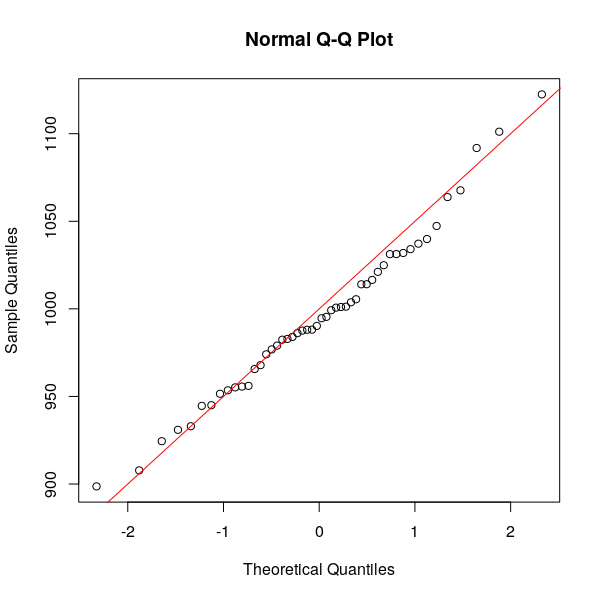
\includegraphics[width=.45\textwidth]{sampling-qqplot-good.png}
  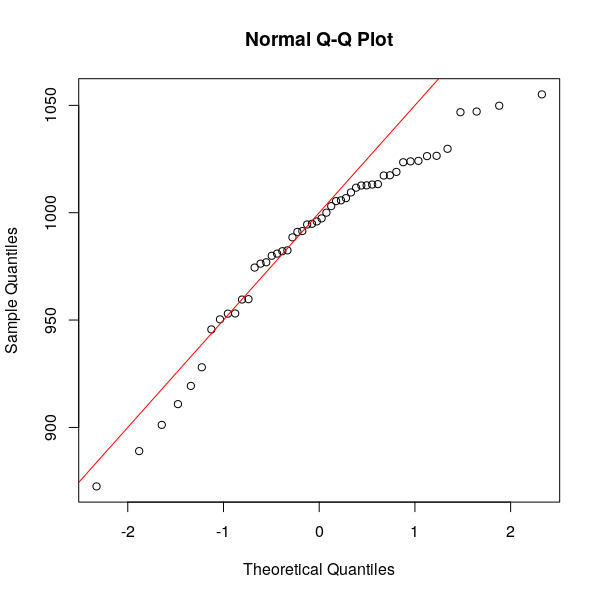
\includegraphics[width=.45\textwidth]{sampling-qqplot-bad.png}
  \end{center}
  \caption{The Q-Q plot on the left is based on a sample of 50 observations drawn from a normal distribution with mean 1000 and standard deviation of 50. The one on the right is based on a sample of 50 observations drawn from Student's $t$ distribution with 15 degrees of freedom, with the same mean and standard deviation. The lines in red are where the observations should theoretically be situated. In the plot on the left, this is more or less the case, but on the right, especially in the extremes, observations deviate from the line.}
  \label{fig:qqplot}
\end{figure}

\lstinputlisting{data/qqplot.R}

\subsection[The chi-square distribution]{The $\chi^{2}$ distribution}
\label{ssec:chi-square-distribution}

Let $X_{1}, X_{2}, \dots X_{v}$ be independent stochastic variables that are standard normally distributed ($\sim N(0,1)$). The $\chi^{2}$ (chi-square) variable is defined as:

\begin{equation}
  \chi^{2}_{v} = X_{1}^{2} + X_{2}^{2} + \dots + X_{v}^{2} 
\end{equation}

The number $v$ denotes the degrees of freedom\index{degrees of freedom} of the variable. $\chi^{2}$ is a continuous stochastic variable, that is always positive, since it is the sum of squares. The probability density function is:

\[ f_{n}(x) = \frac{1}{2^{\frac{n}{2}}\Gamma(\frac{n}{2})} x^{\frac{n}{2} -1} e^{\frac{x}{2}} \]

The expected value (= mean) is $v$ and variance is $2v$. The mode for $v \geq 2$ is $v-2$.

The $\chi^{2}$ variable does not occur ``in the wild.'' No natural phenomenon can be modelled with this distribution. Nevertheless, it will be quite important further on in this course.

\section{Central limit theorem}
\label{sec:central-limit-theorem}

In this section, we'll discuss one of the most fundamental results in statistics and the foundation of sampling: the central limit theorem.

\begin{theorem}
  A linear combination of a sufficiently large number of independent, identically distributed stochastic variables (i.e. with a well defined expected value and variance) will approximate the normal distribution, regardless the underlying distribution.
\end{theorem}

The proof of this theorem is outside the scope of this course, even though it is surprisingly easy to understand.

\begin{theorem}[The Central limit theorem]
  Consider a random sample of $n$ observations drawn from a population with expected value $\mu$ and standard deviation $\sigma$.
  
  If $n$ is sufficiently large, the probability distribution of the sample mean $\overline{x}$ will approximate a normal distribution with expected value $\mu_{\overline{x}} = \mu$ and standard deviation $\sigma_{\overline{x}} = \frac{\sigma}{\sqrt{n}}$.
  
  The larger the sample, the better the probability distribution of $\overline{x}$ will approximate the expected value of the population, $\mu$.
\end{theorem}

Consequently, when you draw a random sample from independent variables with some unknown distribution, the sample mean will be normally distributed. When we repeat this proces again and again (each time with the same sample size), and record the mean, we approximately obtain the graph of a normal distribution. The larger the sample size, the better the approximation.

What is particularly noteworthy is that the sample mean is normally distributed, regardless the underlying distribution!

This opens the door for a number of applications that are of capital importance to statistics. Particularly, it allows us to draw conclusions for an entire population based only on a subset: a random sample.

\subsection{Application of the central limit theorem}

When drawing a random sample of a sufficiently large size $n$ form a population with an unknown $\mu$ and (known) standard deviation $\sigma$, the probability distribution of the sample mean is a stochastic variable $M \sim N (\overline{x}, \frac{\sigma}{\sqrt{n}})$.

\begin{example}
  Let's consider the reaction time of all our superheroes and assume we have drawn a random sample $n = 100$ and $\overline{x} = 90, \sigma = 60$ (ms).
  
  We can then ask ourselves: what is the probability that the average reaction time of a superhero is below $104$ ms?

  \begin{enumerate}
    \item The stochastic variable here is the average reaction speed $\overline{x}$ in a sample of $n=100$ superheroes. Because of the central limit theory, the following holds:
    \[ \overline{x} \sim Nor(\mu = 90, \sigma_{\overline{x}} = \frac{60}{\sqrt{100}} = 6) \]
    \item We can calculate the associated $z$-score:
    \[ z = \frac{104-90}{\frac{60}{\sqrt{100}}} = \frac{104-90}{6} = 2.33 \]
    \item And therefore: $P(\overline{x} < 104) = P(Z < 2.33) = 1 - 0.0099 \approx 0.99$ or about 99\%
  \end{enumerate}
\end{example}

\subsection{Estimating stochastic parameters}
\label{ssec:estimating-stochastic-parameters}

If we want to study a sample, it is usually with the goal of drawing conclusions with regards to the population as a whole. For example, we want to know the average strength of a superhero, or the fraction of rich superheroes. 

In general, we'll \emph{estimate} a parameter of the population based on the sample. For example, $\overline{x}$ is used as an estimate of $\mu$. This type of estimation is defined as:

\begin{definition}[point estimate]
  A \emph{point estimate}\index{estimate!point} for a population parameter is a formula or equation that allows us to calculate a value to estimate that parameter.
\end{definition}

Another type of estimates are the \emph{interval estimates}\index{estimate!interval}, a.o.~confidence intervals. These are discussed in the next sections.

\subsection{Confidence interval for population mean for a large sample}
\label{ssec:confidence-interval-pop-mean-large-sample}

When we estimate the population mean from a sample, we have no idea how correct this estimate is. However, the properties of the normal distribution allow us to construct an interval that will contain the population mean with the desired level of confidence.

\begin{definition}[Confidence interval]
  A \emph{Confidence interval}\index{confidence interval} is an equation or formula that allows us to construct an interval that will contain the parameter to be estimated with a certain level of confidence.
\end{definition}

An initial estimate for the population mean is of course the sample mean:

\[ \overline{x} = \frac{1}{n} \sum_{i} x_{i} \]

Of course this estimate is not the real population mean. However, because of the central limit theorem, we know that the mean of a sample of size $n$ is normally distributed with mean $\mu$ and standard deviation $\frac{\sigma}{\sqrt{n}}$

After standardisation, we get:
\[ Z = \frac{\overline{x} - \mu}{\frac{\sigma}{\sqrt{n}}} \]
This expression depends on $\mu$, but we know that it's normally distribution. That means that we can find limits $-z$ and $z$, independent from $\mu$, that will contain $Z$ with a confidence level $1 - \alpha$ that can be chosen by the researcher. In this example, we choose $1 - \alpha= 0.95$ (and consequently $\alpha = 0.05$).
\[P(-z < Z < z) = 1 - \alpha = 0.95 \]
By applying the rule of symmetry, we find that we need to determine $z$ with:
\[ P( Z < z) = 0.975 \]
When we look this up in a Z-table, we'll find $z = 1.96$. Or, alternatively, we can calculate \verb|qnorm(0.975)| in R.

The confidence interval then is:
\[ P( -1.96 < \frac{\overline{x} - \mu}{\frac{\sigma}{\sqrt{n}}} < 1.96 ) = 1 - \alpha\]
and so
\[ P ( \overline{x} -1.96 \frac{\sigma}{\sqrt{n}} <\mu < \overline{x} + 1.96 \frac{\sigma}{\sqrt{n}}) = 1 - \alpha \]

With this technique, we can determine the bounds of an interval that will contain $\mu$ with confidence level of 95\%. If you would repeatedly draw a sample from this population and calculate the confidence interval around $\overline{x}$, then in 95\% of the cases, we expect the actual $\mu$ to be inside of the interval bounds.

Remark that we assume to know the standard deviation of the population, which is generally not the case. If the sample size is sufficiently large, the sample standard deviation is used as a point estimate for the population standard deviation.

\[ P ( \overline{x} -1,96 \frac{\sigma_{\overline{x}}}{\sqrt{n}} < \mu < \overline{x} + 1,96 \frac{\sigma_{\overline{x}}}{\sqrt{n}}) = 1 - \alpha \]


\begin{figure}
\centering
\begin{tikzpicture}
\begin{axis}[
  domain=-3:3, samples=100,
  axis lines*=left, xlabel=$z$,
  every axis y label/.style={at=(current axis.above origin),anchor=south},
  every axis x label/.style={at=(current axis.right of origin),anchor=west},
  height=5cm, width=12cm,
  xtick={-1.96,0,1.96}, ytick=\empty,
  enlargelimits=false, clip=false, axis on top,
  grid = major
  ]
  \addplot [fill=cyan!20, draw=none, domain=-3:3] {gauss(0,1)} \closedcycle;
  \draw [yshift=-0.6cm, latex-latex](axis cs:-1.96,0) -- node [fill=white] {$\sigma$} (axis cs:1.96,0);
\end{axis}
\end{tikzpicture}
\caption{Standaardnormale verdeling die 95\% betrouwbaarheidsinterval aanduidt.}
\label{fig:verdelingStandaardnormaal}
\end{figure}

\subsection{Confidence interval for population mean for a small sample}
\label{ssec:confidence-interval-pop-mean-small-sample}

In the case of small samples, we can no longer assume that the probability distribution of $\overline{x}$ approximates the normal distribution. The central limit theorem only holds for sample sizes of about $n > 30$.

The shape of the probability distribution of $\overline{x}$ now depends of the shape of the underlying probability distribution of the population. Even thoug $\sigma_{\overline{x}} = \frac{\sigma}{\sqrt{n}}$ still holds, the sample standard deviation $s$ may be a bad estimate for $\sigma$ if the sample is small.

However, there is a solution in the form of the so-called Student's $t$ distribution. Instead of:
\[ z = \frac{\overline{x} - \mu}{\frac{\sigma}{\sqrt{n}}} \]
we use the $t$-score:
\[ t = \frac{\overline{x} - \mu}{\frac{s}{\sqrt{n}}} \]

The probability density of Student's $t$ distribution is very similar to the standard normal distribution: bell-shaped, symmetrical, and with an expected value of 0.

The exact shape depends on the sample size $n$, or more precisely on the degrees of freedom\index{degrees of freedom} $(n-1)$ (abbreviated to $df$).

Remark that:
\begin{itemize}
  \item $(n-1)$ was also used to calculate the sample variance $s^{2}$;
  \item When $n \rightarrow \infty$ this converges to the standard normal distribution.
\end{itemize}

In order to calculate a confidence interval for a sample with a small number of observations, we need to do the determine:
\[ \overline{x} \pm t_{\frac{\alpha}{2}}\left(\frac{s}{\sqrt{n}}\right) \]
with $t_{\frac{\alpha}{2}}$ based on $(n-1)$ degrees of freedom. We still assume that the sample is random and drawn from a population that is approximately normally distributed.

\subsection{Confidence interval for population fraction for a large sample}
\label{ssec:confidence-interval-pop-fraction-large-sample}

If you want to measure a variable as a fraction, for example the percentage of people that responded with ``yes'' to a specific question, this is equivalent to estimating the probability $p$ on success in a binomial experiment, i.e.~an experiment with a sample space consisting of two elements, ``success'' and ``failure''. If the probility of ``success'' is $p$, the probability of ``failure'' is $q = 1 - p$. The value of $p$ can be estimated from the sample:

\[ \overline{p} = \frac{\textnormal{number of successes}}{n} \]

In order to calculate a confidence interval for $\overline{p}$, we need to know the probability distribution of $\overline{p}$. The central limit theory can then be applied to the average number of successes in a sample of size $n$. The probability distribution of $\overline{p}$ has the following properties:

\begin{itemize}
  \item Expected value of the probability distribution of  $\overline{p}$ is $p$.
  \item The standard deviation of the probability distribution of $\overline{p}$ is $\sqrt{\frac{pq}{n}}$
  \item For large samples, $\overline{p}$ is approximately normally distributed.
\end{itemize}

Since $\overline{p}$ is the sample mean of the number of successes, this allows us to calculate a confidence interval, analougous to the one for $\overline{x}$ for large samples.

\begin{definition}[Confidence interval for $p$ for a large sample]
  \[ \overline{p} \pm z_{\frac{\alpha}{2}} \sqrt{\frac{\overline{p}\overline{q}}{n}} \]
  with $\overline{p} = \frac{x}{n}$ and $\overline{q} = 1- \overline{p}$
\end{definition}

